%%% Preamble
\documentclass{report}

\usepackage[utf8]{inputenc}
\usepackage[T1]{fontenc}
\usepackage{fourier}
\usepackage[french]{babel}
\usepackage[protrusion=true,expansion=true]{microtype}	
\usepackage{amsmath,amsfonts,amsthm} % Math packages
\usepackage[pdftex]{graphicx}	
\usepackage{url}
\usepackage{pdfpages}
\usepackage{todonotes}
\usepackage[a4paper, body={16cm,26cm}]{geometry}
\usepackage{float}
\usepackage{framed}
\usepackage[toc,page]{appendix} 
\usepackage{multicol}
\usepackage{colortbl}
\usepackage{epstopdf}
\usepackage{adjustbox}

%%% Custom sectioning
\usepackage{sectsty}
\allsectionsfont{  \normalfont\scshape}
%\allsectionsfont{\centering \normalfont\scshape}

%%% Custom headers/footers (fancyhdr package)
\usepackage{fancyhdr}
\pagestyle{fancyplain}
\fancyhead{}								% No page header
\fancyfoot[L]{}							% Empty 
\fancyfoot[C]{}							% Empty
\fancyfoot[R]{\thepage}					% Pagenumbering
\renewcommand{\headrulewidth}{0pt}		% Remove header underlines
\renewcommand{\footrulewidth}{0pt}		% Remove footer underlines
\setlength{\headheight}{13.6pt}


%%% Equation and float numbering
\numberwithin{equation}{section}		% Equationnumbering: section.eq#
\numberwithin{figure}{section}		% Figurenumbering: section.fig#
\numberwithin{table}{section}		% Tablenumbering: section.tab#


%%% Define new commands
\newcommand{\horrule}[1]{\rule{\linewidth}{#1}} 	% Horizontal rule
\renewcommand{\bf}[1]{\textbf{#1}}
\renewcommand{\it}[1]{\textit{#1}}
\newcommand{\bfit}[1]{\textbf{\textit{#1}}}
\renewcommand{\sc}[1]{\textsc{#1}}

\newcommand{\Todo}[1]{\todo[inline]{#1}}
\renewcommand{\thesection}{\thepart .\arabic{section}}

\usepackage{tocloft}
\cftsetindents{chapter}{0em}{1em}
\cftsetindents{section}{1.5em}{2.5em}
\makeatletter
\def\l@figure{\@dottedtocline{1}{1.5em}{4em}}
\makeatother

\usepackage{bookmark}
%\usepackage[hidelinks]{hyperref}
\usepackage{cases}
\usepackage{color}
\usepackage{xcolor}
\usepackage{relsize}
\usepackage{caption}
\colorlet{shadecolor}{black!10}

\delimitershortfall-1sp
\newcommand\abs[1]{\left|#1\right|}


\usepackage{tikz, pgfplots}


%}}}
%{{{ --- pgfplots ---------------------

%{{{ Colors

% TolColors from http://www.r-bloggers.com/the-paul-tol-21-color-salute/
\definecolor{TolColor1}{HTML}{332288}   % dark purple
\definecolor{TolColor2}{HTML}{6699CC}   % dark blue
\definecolor{TolColor3}{HTML}{88CCEE}   % light blue
\definecolor{TolColor4}{HTML}{44AA99}   % light green
\definecolor{TolColor5}{HTML}{117733}   % dark green
\definecolor{TolColor6}{HTML}{999933}   % dark brown
\definecolor{TolColor7}{HTML}{DDCC77}   % light brown
\definecolor{TolColor8}{HTML}{661100}   % dark red
\definecolor{TolColor9}{HTML}{CC6677}   % light red
\definecolor{TolColor10}{HTML}{AA4466}  % light pink
\definecolor{TolColor11}{HTML}{882255}  % dark pink
\definecolor{TolColor12}{HTML}{AA4499}  % light purple

%}}}
%{{{ Color cycles

\pgfplotscreateplotcyclelist{mbarplot cycle}{%
  {draw=TolColor2, fill=TolColor2!70},
  {draw=TolColor7, fill=TolColor7!70},
  {draw=TolColor4, fill=TolColor4!70},
  {draw=TolColor11, fill=TolColor11!70},
  {draw=TolColor1, fill=TolColor1!70},
  {draw=TolColor8, fill=TolColor8!70},
  {draw=TolColor6, fill=TolColor6!70},
  {draw=TolColor9, fill=TolColor9!70},
  {draw=TolColor10, fill=TolColor10!70},
  {draw=TolColor12, fill=TolColor12!70},
  {draw=TolColor3, fill=TolColor3!70},
  {draw=TolColor5, fill=TolColor5!70},
}

\pgfplotscreateplotcyclelist{mlineplot cycle}{%
  {TolColor2, mark=*, mark size=1.5pt},
  {TolColor7, mark=square*, mark size=1.3pt},
  {TolColor4, mark=triangle*, mark size=1.5pt},
  {TolColor6, mark=diamond*, mark size=1.5pt},
}


\pgfplotsset{
  compat=1.9,
  mbaseplot/.style={
    legend style={
      draw=none,
      fill=none,
      cells={anchor=west},
    },
    x tick label style={
      font=\footnotesize
    },
    y tick label style={
      font=\footnotesize
    },
    legend style={
      font=\footnotesize
    },
    major grid style={
      dotted,
    },
    axis x line*=bottom,
  },
  mlineplot/.style={
    mbaseplot,
    xmajorgrids=true,
    ymajorgrids=true,
    major grid style={dotted},
    axis x line=bottom,
    axis y line=left,
    legend style={
      cells={anchor=west},
      draw=none
    },
    cycle list name=mlineplot cycle,
  },
  mbarplot base/.style={
    mbaseplot,
    bar width=6pt,
    axis y line*=none,
  },
  mbarplot/.style={
    mbarplot base,
    ybar,
    xmajorgrids=false,
    ymajorgrids=true,
    area legend,
    legend image code/.code={%
      \draw[#1] (0cm,-0.1cm) rectangle (0.15cm,0.1cm);
    },
    cycle list name=mbarplot cycle,
  },
  horizontal mbarplot/.style={
    mbarplot base,
    xmajorgrids=true,
    ymajorgrids=false,
    xbar stacked,
    area legend,
    legend image code/.code={%
      \draw[#1] (0cm,-0.1cm) rectangle (0.15cm,0.1cm);
    },
    cycle list name=mbarplot cycle,
  },
  disable thousands separator/.style={
    /pgf/number format/.cd,
      1000 sep={}
  },
}


%%  ========   IMPORTANT ========
%% Spécifier ici les variables pour le document
\newcommand{\mainTitle}{\'Etude préalable - SPIE}
\newcommand{\secondTitle}{Document de suivi}
\newcommand{\documentRef}{TB/4401/1}
\newcommand{\auteurs}{
Paul \textsc{Dautry}
}
\newcommand{\chefDeProjet}{Paul \textsc{Dautry}}
\newcommand{\responsableQualite}{Antoine \textsc{Chabert}}

%%% Begin document
\begin{document}
%----------------------------------------------------------------------------------------
%	PACKAGES
%----------------------------------------------------------------------------------------

\documentclass[12pt]{article}
\usepackage[a4paper]{geometry}
\geometry{verbose,tmargin=1in,bmargin=0in,lmargin=1in,rmargin=1in}
\usepackage[utf8]{inputenc}
\usepackage[francais]{babel}
\usepackage[T1]{fontenc}

\usepackage{graphicx}
\begin{document}

\begin{titlepage}

\newcommand{\HRule}{\rule{\linewidth}{0.5mm}} % horizontal lines

\center % Center everything
 
%----------------------------------------------------------------------------------------
%	HEADING SECTIONS
%----------------------------------------------------------------------------------------

\vspace*{1cm}

\textsc{\LARGE INSA de LYON}\\[1.5cm] 
\textsc{\Large D\'epartement Informatique}\\[0.5cm] 
\textsc{\large Projet Longue Durée}\\[0.5cm] % 

%----------------------------------------------------------------------------------------
%	TITLE SECTION
%----------------------------------------------------------------------------------------

\HRule \\[0.4cm]
{ \huge \bfseries Compte Rendu}\\[0.1cm]
{\large \bfseries - Gestion des contacts commerciaux d'une banque -} 
\HRule \\[1.5cm]
 
%----------------------------------------------------------------------------------------
%	DATE SECTION
%----------------------------------------------------------------------------------------

{\large \today}\\[2cm] % 
 
%----------------------------------------------------------------------------------------
%	AUTHOR SECTION
%----------------------------------------------------------------------------------------

\begin{minipage}{0.4\textwidth}
\begin{center} \large
\emph{Auteurs} \\
Lisa \textsc{Courant} \\
Estelle \textsc{Lepeigneux} \\
Pierre \textsc{Jarsaillon} \\
Hugues \textsc{Verlin} \\
\end{center}
\end{minipage}
~
\begin{minipage}{0.4\textwidth}
\begin{center} \large
\emph{Chef de projet} \\
Paul \textsc{Dautry}
\end{center}
\begin{center} \large
\emph{Responsable Qualité} \\
Antoine \textsc{Chabert}
\end{center}
\end{minipage}\\[5cm]

H4401\\[2cm]

%----------------------------------------------------------------------------------------
%	LOGO SECTION
%----------------------------------------------------------------------------------------

\includegraphics[scale=0.3]{figures/logo.png}
%----------------------------------------------------------------------------------------

\vfill % Fill the rest of the page with whitespace

\end{titlepage}
\end{document}


%% Commenter les deux lignes suivantes pour le document final
%\listoftodos
\newpage

%% Table de matière / figures / tableaux
\tableofcontents
\listoffigures
\listoftables
\newpage


\part{Bilan phase d'Initialisation}

Ce bilan a été rédigé le 13 décembre 2015. Le tableau de bord associé est pésent en Annexe A.

\setcounter{section}{0}

\section{Bilan d'avancement}

Au terme de cette séance d'initialisation, l'ensemble des tâches a été réalisé dans les temps. Il n'y a donc pas, à ce stade, de glissement concernant le planning. L'ajout des exercices ARIS à quelque peu perturbé le programme mais cette perturbation à été très bien absorbé par le travail efficace mené par les membres de l'équipe. Il a cependant été décidé de mettre de côté certains exercices pour dégager conserver du temps pour réaliser les tâches que l'on pourrait qualifier de principales. Les indicateurs concernant les livrables sont donc verts. \\

Du point de vue de la gestion de la qualité, la vérification de la bonne application des règles énoncées dans le PAQ est réalisée à chaque séance sous la forme de revues des livrables et des différents documents en production. Ces tâches se révèlent utiles dans le sens où l'on constate parfois quelques dérives au niveau de l'utilisation des outils collaboratifs qui pourraient conduire à un certain désordre si ces vérifications n'étaient pas effectuées. \\

Pour finir, les tâches de gestion de projet sont menées régulièrement afin de guider, au mieux, les membres de l'équipe. La définition des tâches n'est pas une tâche facile et il est difficile d'atteindre une granularité suffisante sur des tâches pour lesquelles la visibilité n'est pas bonne (tâches temporellement lointaine et/ou floue). Un travail de mise à jour des tâches est donc effectué la veille de chaque séance afin d'assurer une définition suffisante des tâches pour que les membres n'aient pas à se poser de question et puissent se contenter de réaliser ou de suivre la réalisation des tâches qui sont sous leur responsabilité. \\

\section{Bilan humain}

D'un point de vue humain on note une baisse dans le moral des membres de l'équipe il est en effet difficile de motiver les membres qui sont pour la plupart déçus des problèmes, récurrents, d'accès aux ressources. De même, ils estiment que la durée de travail recommandée en dehors des heures de projet est largement sous-estimée. \\
Il est malheureusement impossible d'envisager des actions correctives car ces problèmes ne peuvent pas être résolu par nos soins.


\part{Bilan phase d'Expression du Besoin - \'Etude de l'\'Existant}

Ce bilan a été rédigé le 18 décembre 2015. Le tableau de bord associé est pésent en Annexe B.

\setcounter{section}{0}

\section{Bilan d'avancement}

Les tâches concernant l'étude de l'existant ont été partiellement réaisées et se sont révélées plus longues, en effet, l'analyse des différents processus prends un certain temps et la plateforme ARIS a été inaccessible la plupart du temps pendant les séance de projet. Cette même plateforme n'est pas accessible à l'extérieur de l'INSA et ne peut donc être utilisée que dans les salles de TP. Les causes de ce problème sont identifiées mais, de nouveau, sont indépendantes de notre volonté. Un seul membre de l'hexanome est parvenu, après plus de 2h de bataille, à faire fonctionner l'application dans un environnement technique particulier ne permettant pas à tous les membres de l'hexanome d'en faire de même (enivronnement d'exécution propriétaire). \\

Concernant la qualité, les tâches se limitent à vérifier le bon usage des outils et la qualité du contenu et des recherches effectuées. Aucun livrable n'a encore été constitué. \\

La gestion de projet, quant à elle, consiste à réaliser le suivi des indicateurs et animer les réunions. Il est également nécessaire de mettre à jour la liste des tâches et l'avancement de ces dernières. La vérification du bon usage du tableau de bord, notamment la saisie des temps, est aussi une des activités exercée lors des séances de projet. La rédaction de ce bilan hebdomadaire permet de prendre du recul sur le travail accompli et le travail restant. \\

\section{Bilan humain}

Vu le peu d'amélioration concernant les conditions d'accès aux outils de travail, le moral continue de chuter. Espérons que cette situation ait trouvée une réponse après les vacances et que ces dernières aient permis aux membres de l'équipe de se ressourcer pour reprendre le projet dans les meilleures conditions. Il est également difficile en tant que chef de projet de faire en sorte que l'équipe se sentent concernée par le projet si les tâches qui leurs sont affectées ne peuvent être réalisées.


\part{Bilan phase d'Expression du Besoin - Benchmarking}

Ce bilan a été rédigé le 8 janvier 2016. Le tableau de bord associé est pésent en Annexe C.

\setcounter{section}{0}

\section{Bilan d'avancement}

La poursuite de la réalisation des tâches de l'étude de l'existant est effectuée en paralèlle de l'initialisation des taches de la phase de benchmarking. Le benchmarking nécessite selon nos estimations moins de temps de travail et le déséquilibre entre l'étude de l'existant et le benchmarking en terme de charge de travail se ressent par un léger glissement sur le planning. Ce glissement n'est pas important mais nous apporterons une attention particulière afin de veiller à ce que celui-ci ne s'aggrave pas. Nous serons dans les temps pour fournir les livrables attendus.

Des facteurs extérieurs ayant décalé la réalisation de l'exercice SAP par l'équipe celui-ci n'a pu être réalisé pendant cette phase et a été rendu au moment de la reprise du projet après la période des fêtes. La date de rendu n'ayant pas été modifiée, le document est considéré comme étant rendu en retard ce qui n'est pas de notre fait, nous tenons à le préciser.

Concernant la qualité, les tâches se limitent à vérifier le bon usage des outils et la qualité du contenu et des recherches effectuées. Des livrables sont en cours de constitution et leur constitution progressive facilite le travail de releecture par l'intégration progressive. \\

La gestion de projet, quant à elle, consiste à réaliser le suivi des indicateurs et animer les réunions. Des efforts conséquents ont été fourni afin de guider au mieux les membres de l'équipe dans leur travail afin de garantir une certaines efficacité pour tenter de compenser le glissement occasionné par l'indisponibilité de certaines ressources essentielles pour la réalisation de l'étude. Il est, comme d'ordinaire, toujours nécessaire de mettre à jour la liste des tâches et l'avancement de ces dernières. Le tableau de bord est surveillé et mis à jour lors des séances de projet et des contrôles de cohérence sont effectués à chaque séance. Ce bilan est rédigé comme d'ordinaire sur le temps de la séance. \\

\section{Bilan humain}

L'accès au ressources n'est toujours pas rétablit mais certaines tâches peuvent tout de même être menées. L'équipe fait des efforts et fournit un travail important comparé à la charge anoncée initialement. Tout n'est pas dimmensionné à la perfection et ce malgré le moral. Nous esperons que les conditions s'améliorerons après la période des fêtes. Ce bilan étant rédigé après la période précédement citée il est d'ors et déjà possible de dire que l'accès au ressources semble être rétablit et stable mais les congés n'ont pas fourni le repos nécessaire à l'équipe.


\part{Bilan phase d'Expression du Besoin - Spécification de la cible fonctionnelle}

Ce bilan a été rédigé le 12 janvier 2016. Le tableau de bord associé est pésent en Annexe D.

\setcounter{section}{0}

\section{Bilan d'avancement}

Le retard accumulé ayant provoqué un glissement relativement important dans le planning des tâches s'est résorbé grâce au travail efficace, hors séance, de l'équipe. Nous avons donc réussi à livrer l'ensemble des documents constituant le dossier bilan de la phase d'Expression des Besoins dans les temps. Nous pouvons donc maintenant nous consacrer pleinement à la réalisation des tâches de la phase suivante qui consiste à élaborer deux solutions : une spécifique et une standard basée sur l'utilisation de l'ERP SAP. \\

Les tâches relevant de la qualité se sont diversifiées et comprennent lors de cette courte période la relecture et l'intégration des documents afin de certifier la qualité des livrables qui ont été rendus. Mais également à vérifier le bon usage des outils et notamment du répertoire partagé dans lequel quelques abus ont été constatés et ont rapidement été rectifiés. Les livrables ont été validés et livrés dans les temps ce qui tend à démontrer l'efficacité des processus mis en place dans le PAQ en début de projet malgré les évènements extérieurs ayant quelque peu perturbé le déroulment du projet.\\

Concernant la gestion de projet, les livrables ayant été remis dans les temps malgré un retard conséquent constitue un évènement important dans la vie du projet et justifie les performances des membres de l'équipe et leur efficacité tant sur le plan de l'investissement personnel que du travail de groupe dans lequel aucune tension n'est à déplorer. L'ambiance de travail est saine et l'équipe bien que peu motivée par le projet réalise le travail attendu et comprend de plus en plus l'intérêt de ce dernier au fur et à mesure que le projet avance. Après la validation des livrables, les tâches de gestion de projet vont maintenant se concentrer sur la revue du planning des tâches et la pertinence des tâches définies en début de projet. Il sera également nécessaire de continuer à effectuer des points de synchronisation réguliers qui permettent à l'équipe de se situer.

\section{Bilan humain}

Il semblerait que la période des fêtes n'ait pas été propice au repos des membres de l'équipe qui semblent encore fatigués mais il est possible de sentir un envie commune d'avancer. Le moral n'est pas au plus haut mais nous constatons une certaine stagnation de cet indicateur ce qui signifie que bien que l'évolution ne soit pas positive elle n'empire pas non plus. Tous les membres de l'équipe sont prêts à attaquer la nouvelle phase avec l'envie d'éviter un nouveau glissement. Même si certains membres de l'équipe ne sont pas du tout intéressés par le projet, ils prennent leur responsabilité et effectuent le travail qui leur est demandé ce qui est appréciable. L'ambiance est bonne au sein du groupe.


\part{Bilan phase d'Elaboration des Solutions - Spécification d'une solution spécifique}

Ce bilan a été rédigé le 15 janvier 2016. Le tableau de bord associé est pésent en Annexe E.

\setcounter{section}{0}

\section{Bilan d'avancement}

Concernant les tâches de production, nous avons fait le choix de séparer le groupe en deux afin de développer plus rapidement les deux solutions. Nous avons donc commencé à travailler sur les deux solutions et à l'issue de cette séance, les deux solutions sont initialisées. Le développement de la solution spécifique a atteint la phase de conception des cas d'utilisation. Tandis que la seconde équipe est parvenue à mettre en \oe{}uvre la génération d'un rapport ARIS customisé pour la solution standard et a développé les premiers modèles constituant cette solution. \\

La production de livrables n'étant pas à l'ordre du jour, les tâches de la Qualité consistent principalement en la relecture et l'intégration des documents. Elles consistent toujours à vérifier le bon usage des outils. \\

Concernant la gestion de projet, la phase a commencé par la tenue d'une réunion comme à chaque séance pour faire un point sur ce qui a été réalisé et ce qui doit l'être, le but étant au final de guider un maximum les membres de l'équipe pour que ceux-ci aient des objectifs clairs et puissent mener à bien les tâches qui leur sont confiées. La rédaction du bilan de la séance précédente et le suivi des ndicateurs du tableau de bord font également partie des tâches qui ont été réalisées dans le cadre de la gestion de projet. 

\section{Bilan humain}

Nous notons une légère hausse dans le moral de l'équipe, cette hausse s'explique en partie par l'intérêt que portent les membres à la phase qui vient de débuter. En effet, la majorité des membres de l'équipe sont naturellement attirés par les aspects techniques et la conception de solutions en général. Il est donc naturel de constater une hausse du moral, il sera intéressant de surveiller cet indicateur afin de vérifier que cette hausse se confirme. 


\part{Bilan phase d'Elaboration des Solutions - Spécification d'une solution standard}

Ce bilan a été rédigé le 19 janvier 2016. Le tableau de bord associé est pésent en Annexe F.

\setcounter{section}{0}

\section{Bilan d'avancement}

Concernant les tâches de production, nous avons fait le choix de séparer le groupe en deux afin de développer plus rapidement les deux solutions. Nous avons donc commencé à travailler sur les deux solutions et à l'issue de cette séance, les deux solutions sont initialisées. Le développement de la solution spécifique a atteint la phase de conception des cas d'utilisation. Tandis que la seconde équipe est parvenue à mettre en \oe{}uvre la génération d'un rapport ARIS customisé pour la solution standard et a développé les premiers modèles constituant cette solution. \\

La production de livrables n'étant pas à l'ordre du jour, les tâches de la Qualité consistent principalement en la relecture et l'intégration des documents. Elles consistent toujours à vérifier le bon usage des outils. \\

Concernant la gestion de projet, la phase a commencé par la tenue d'une réunion comme à chaque séance pour faire un point sur ce qui a été réalisé et ce qui doit l'être, le but étant au final de guider un maximum les membres de l'équipe pour que ceux-ci aient des objectifs clairs et puissent mener à bien les tâches qui leur sont confiées. La rédaction du bilan de la séance précédente et le suivi des ndicateurs du tableau de bord font également partie des tâches qui ont été réalisées dans le cadre de la gestion de projet. 

\section{Bilan humain}

Nous notons une légère hausse dans le moral de l'équipe, cette hausse s'explique en partie par l'intérêt que portent les membres à la phase qui vient de débuter. En effet, la majorité des membres de l'équipe sont naturellement attirés par les aspects techniques et la conception de solutions en général. Il est donc naturel de constater une hausse du moral, il sera intéressant de surveiller cet indicateur afin de vérifier que cette hausse se confirme. 


\part{Bilan phase d'Elaboration des Solutions - Configuration de la solution ERP}

Ce bilan a été rédigé le 22 janvier 2016. Le tableau de bord associé est pésent en Annexe G.

\setcounter{section}{0}

\section{Bilan d'avancement}

Concernant les tâches de production, l'équipe s'occupant de la production du rapport pour la solution ARIS a terminé son travail et commence à anticiper les tâches à venir telles que la réalisation de l'évaluation des solutions. Le comparatif des solution n'est pas encore envisageable car la seconde équipe, chargée de la solution spécifique, n'a pas encore totalement fini le dossier présentant cette dernière. Ce dossier sera tout de même terminé pour la séance suivante et livré comme convenu.\\

Les tâches ayant attrait à la Qualité comprennent à la fin de cette phase d'élaboration des solution la relecture et l'intégration des divers documents produits. Elles englobent également les tâches courantes de verification du respect du PAQ.\\

Les tâches de gestion de projet ont été quelques peu limitées pendant cette phase, le Chef de Projet ayant la majorité du temps participé à la constitution du dossier pour la solution spécifique. Les tâches définies pour la phase étant correctes, il n'a pas été nécessaire de les revoir. De plus, la surveillance des indicateurs a été réalisée et aucun situation alarmante ne s'est présentée, aucune action corrective n'a donc été entreprise. L'avancement des livrables est cohérent et il n'y a pas de glissement notable rencontré sur cet fin de phase. Il est clair que les temps ont été surestimés mais il semblerait que les membres ne remplisse pas le tableau de bord avec les durées réelles passées à travailler sur le projet. Une attention particulière sera portée sur ce point lors des prochaines séances.

\section{Bilan humain}

Un des membres est malade, ce risque était prévu dans le PAQ. Ceci ne pose pas de problème sachant que la solution standard est terminée et que ce membre faisait partie de cette équipe. La hausse concernant le moral se confirme. Aucune action corrective n'est donc à envisager. La fin du projet approche et les membres s'investissent de manière importante il est donc intéressant de constater qu'il n'y a pas d'essoufflement sur la durée.



\begin{appendices}

\chapter{Tableau de Bord le 13/12/2015}
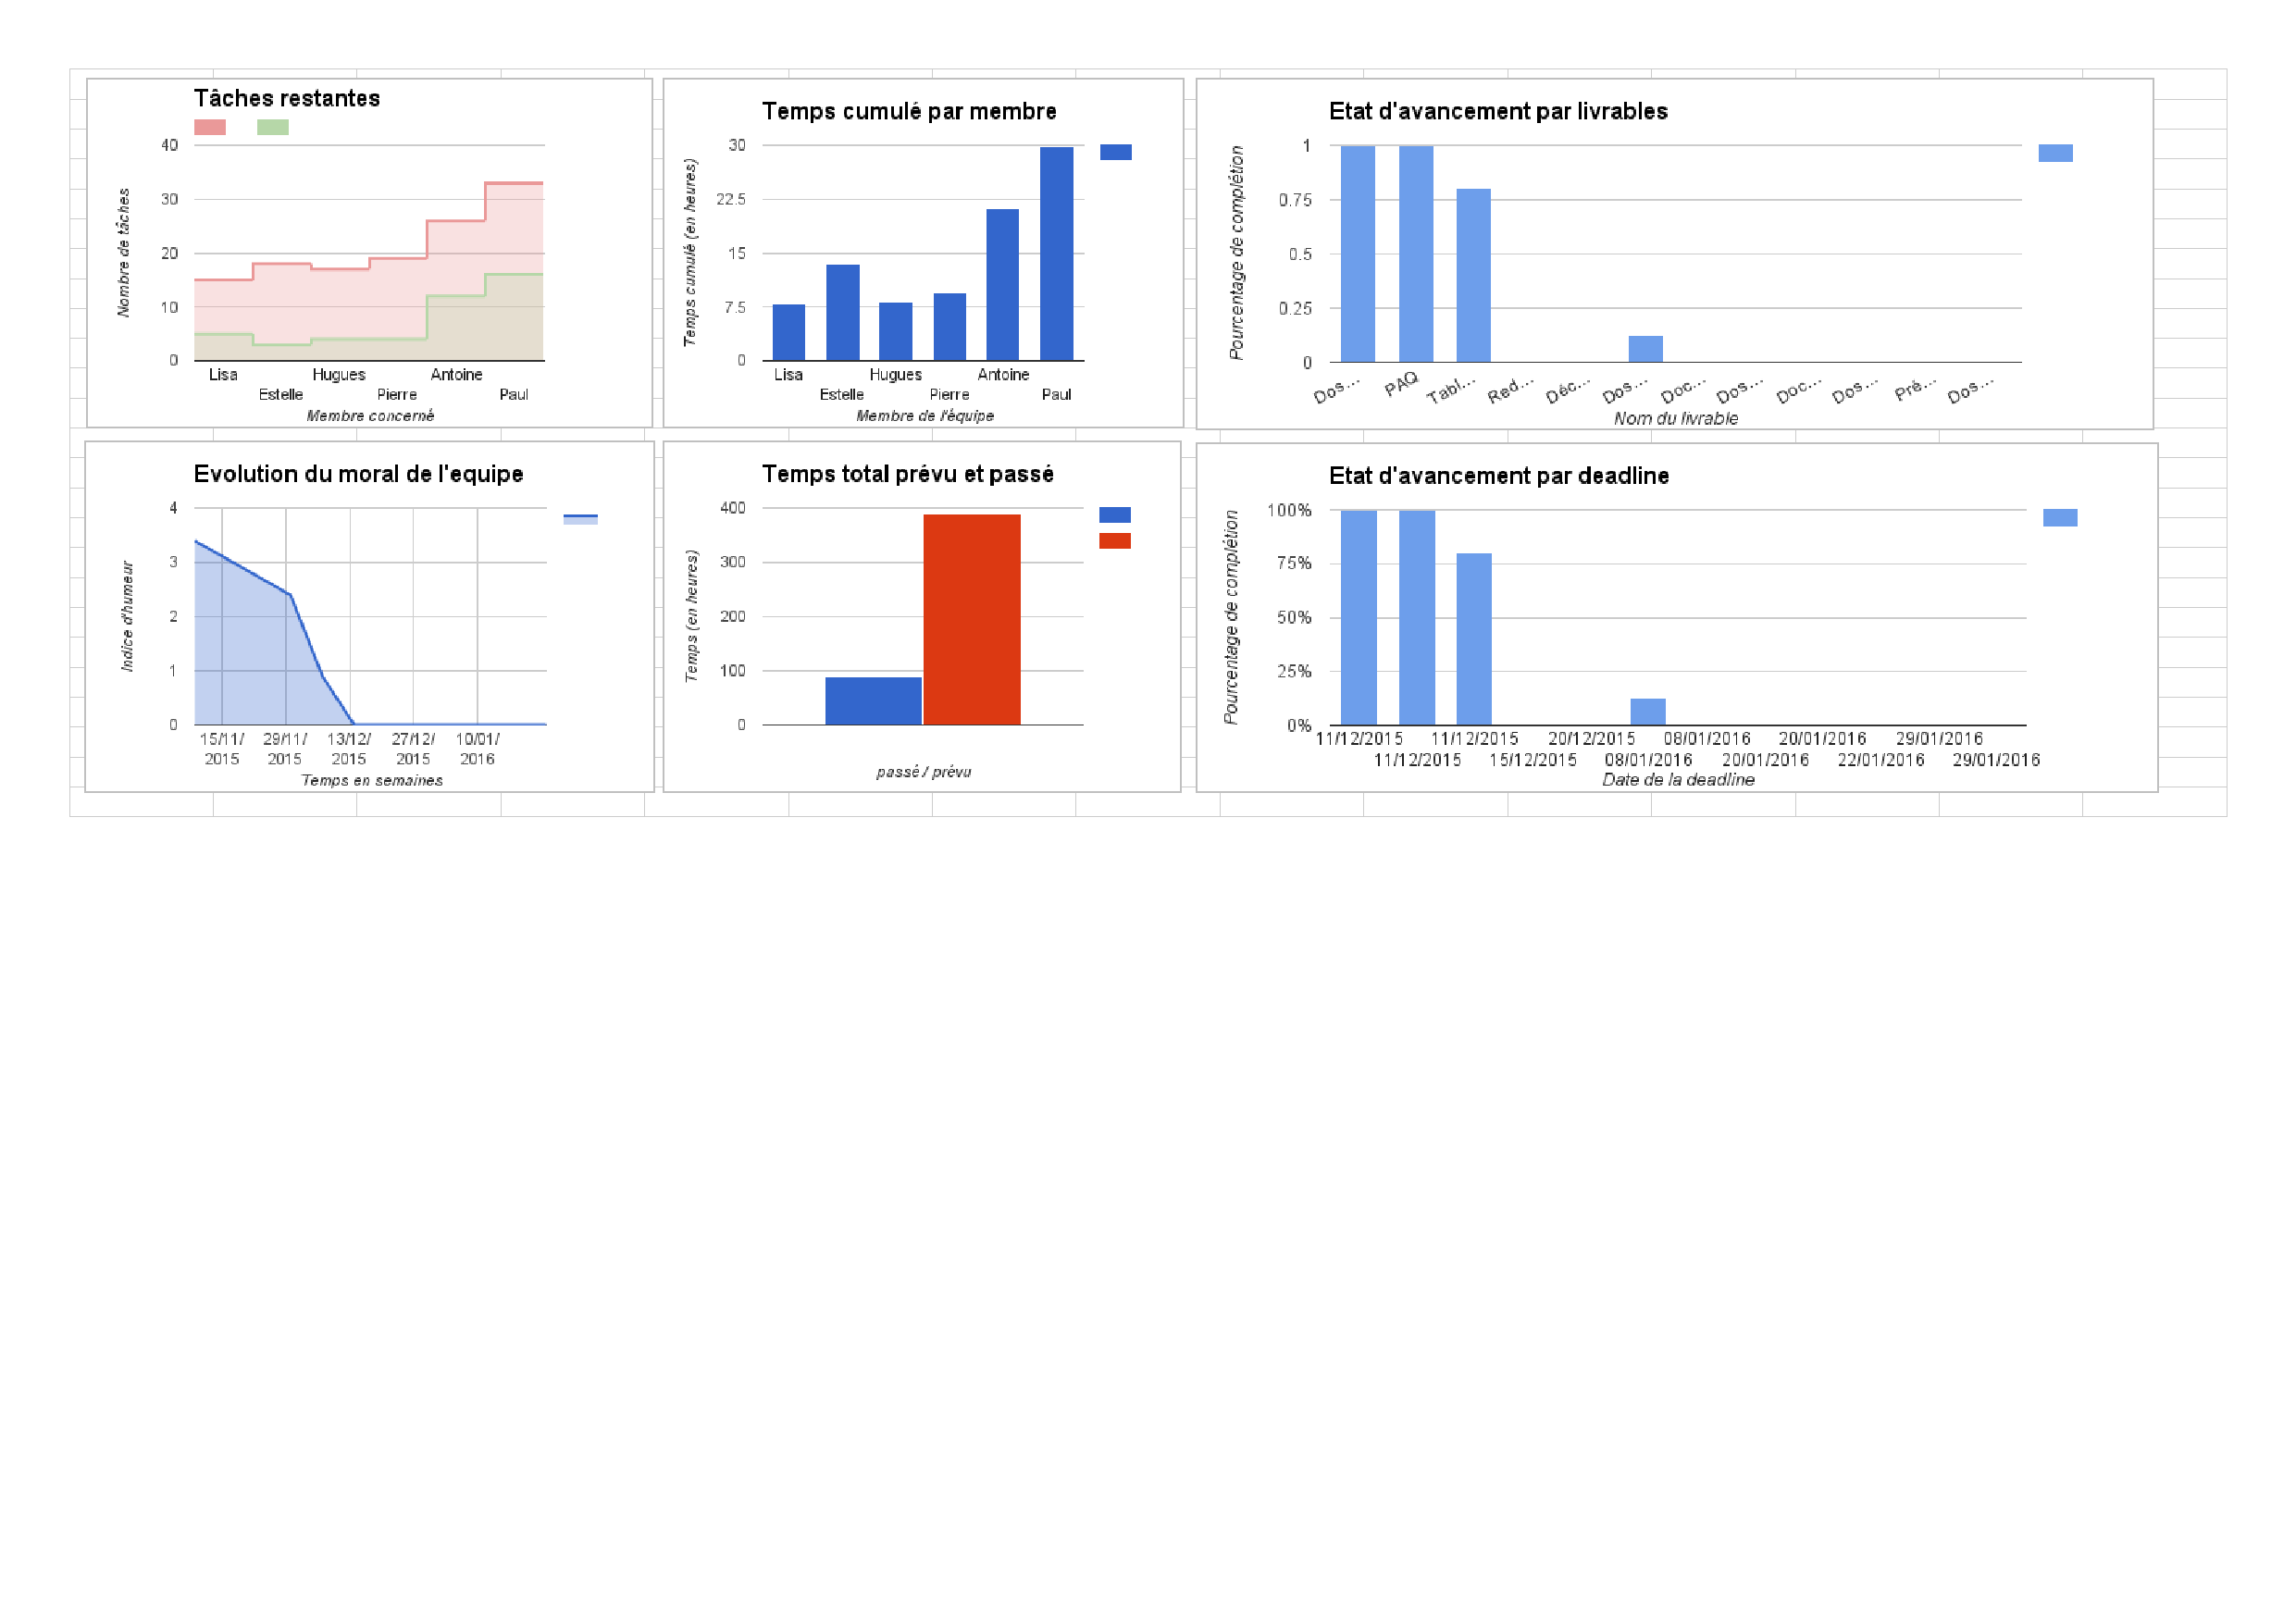
\includepdf[pages=-]{tdbs/Tableau_de_Bord_13-12-15.pdf}

\chapter{Tableau de Bord le 18/12/2015}
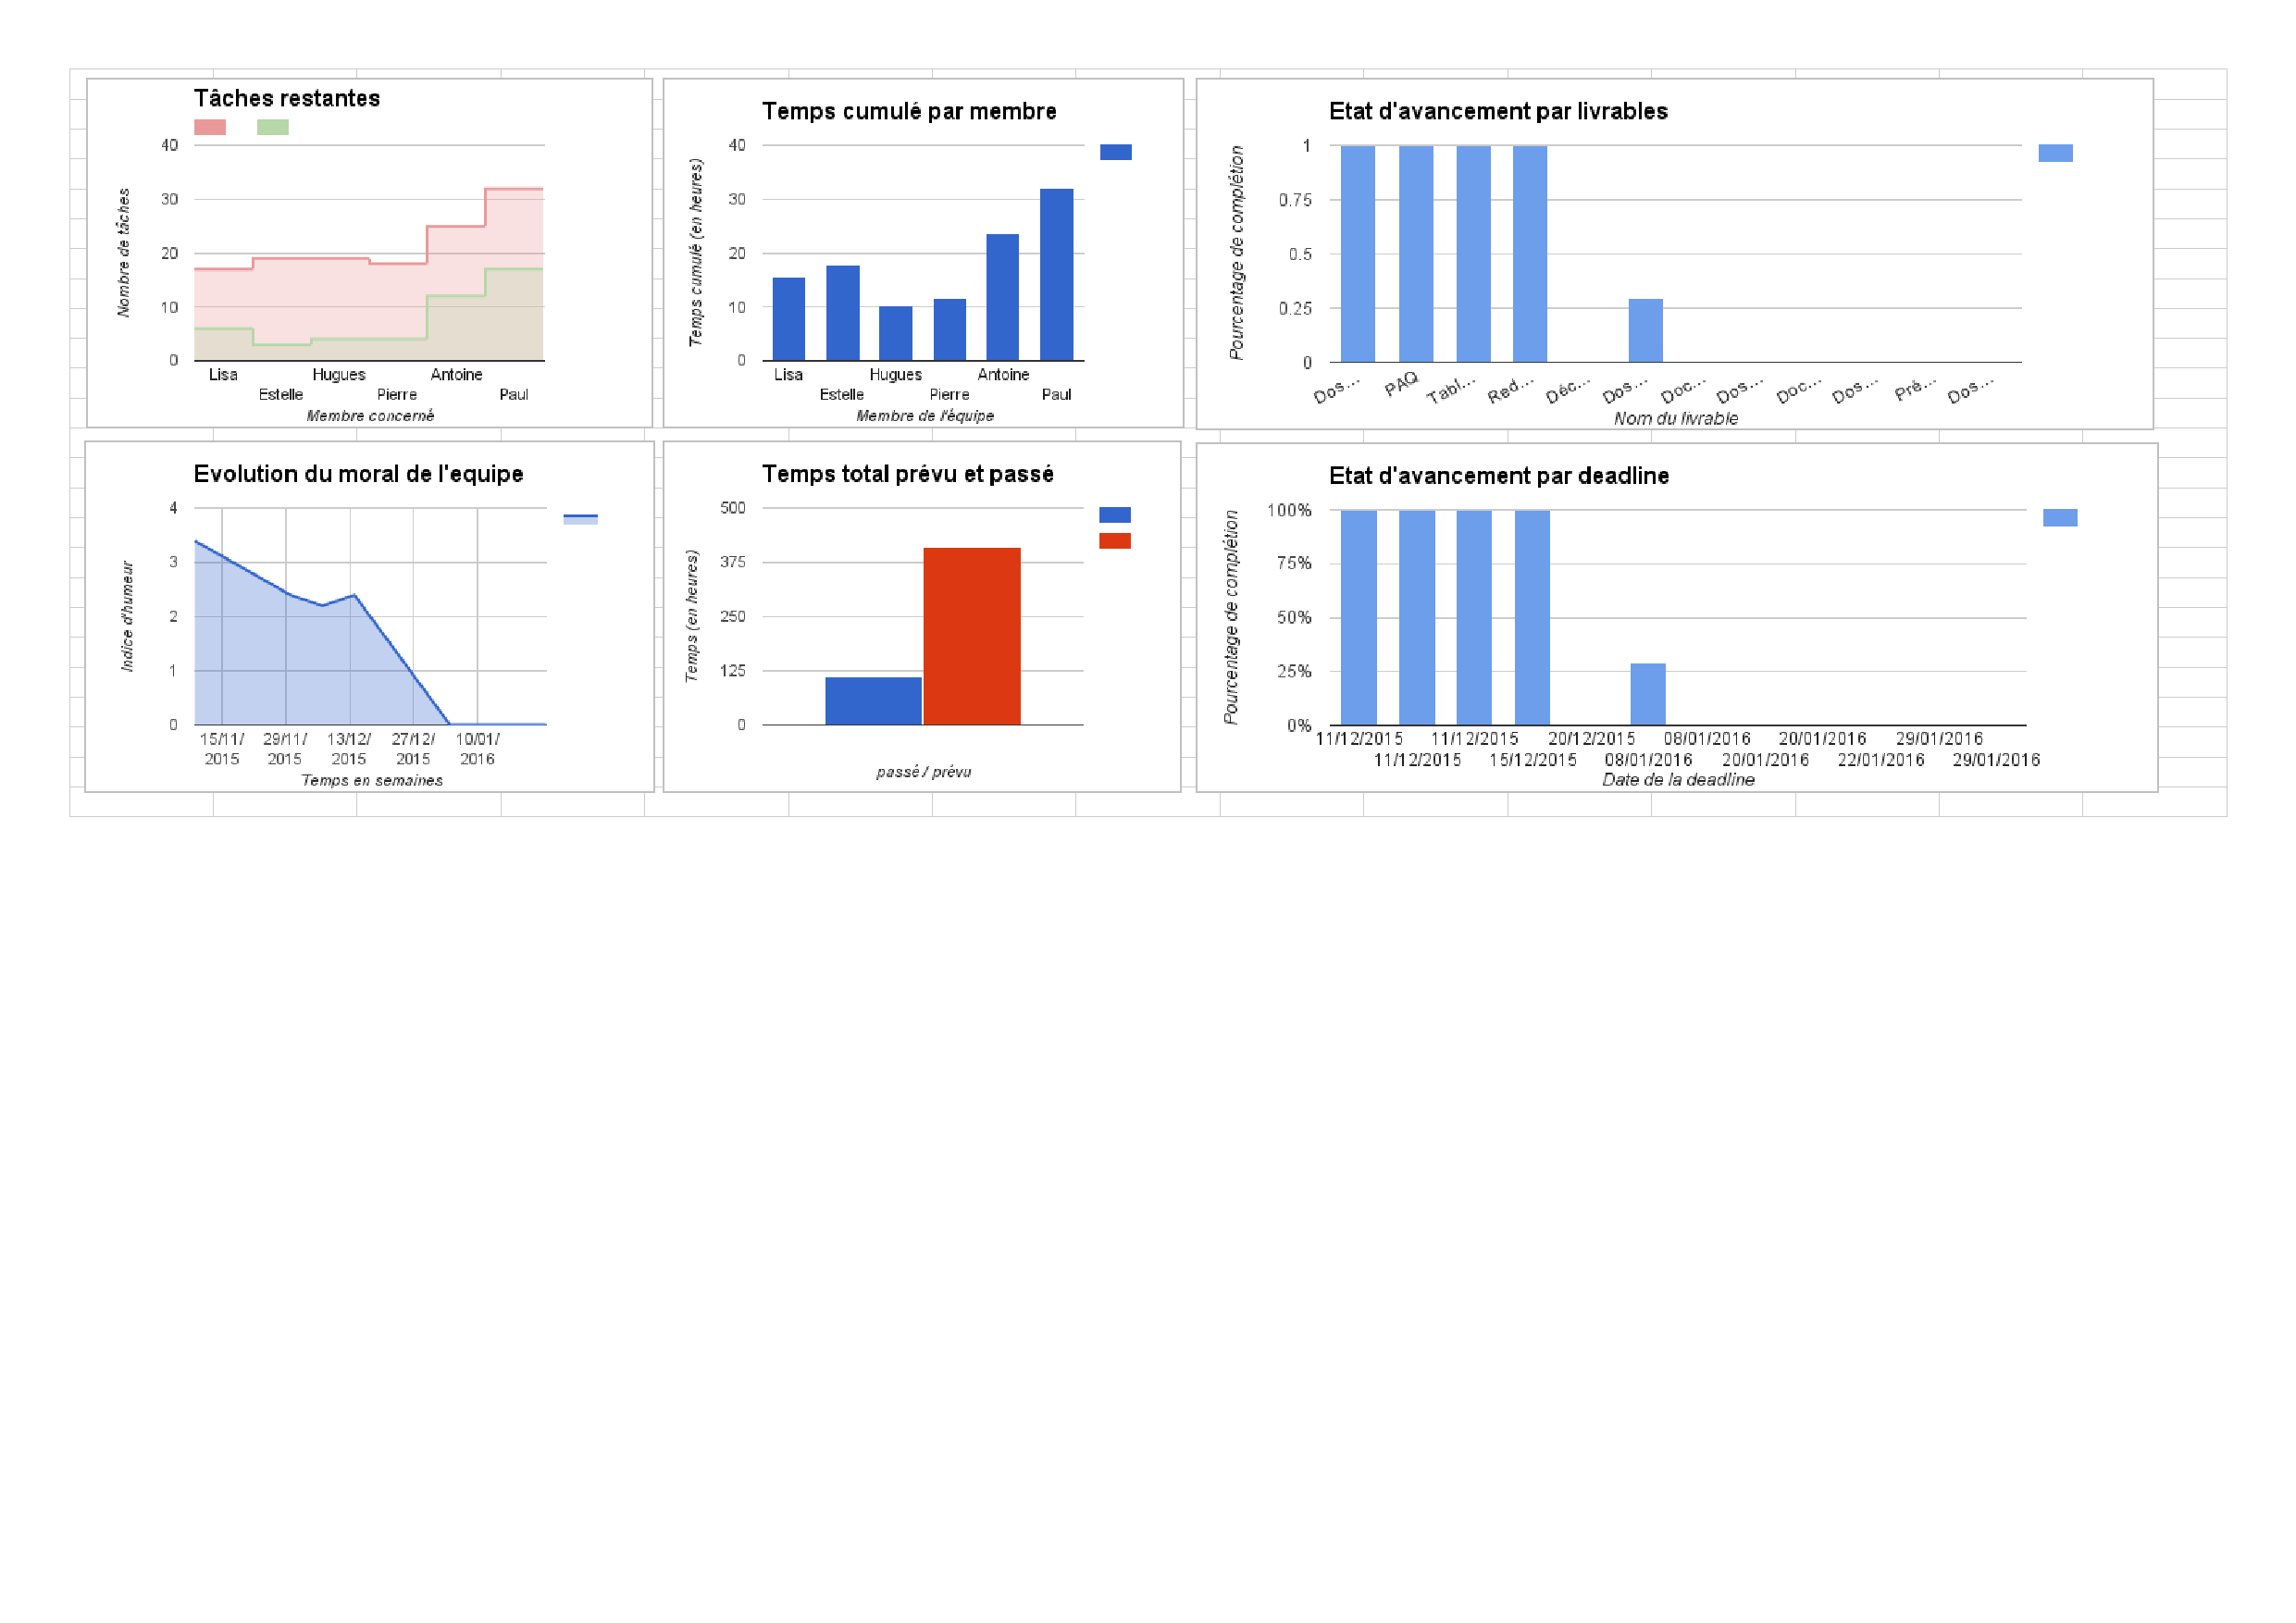
\includepdf[pages=-]{tdbs/Tableau_de_Bord_18-12-15.pdf}

\chapter{Tableau de Bord le 08/01/2016}
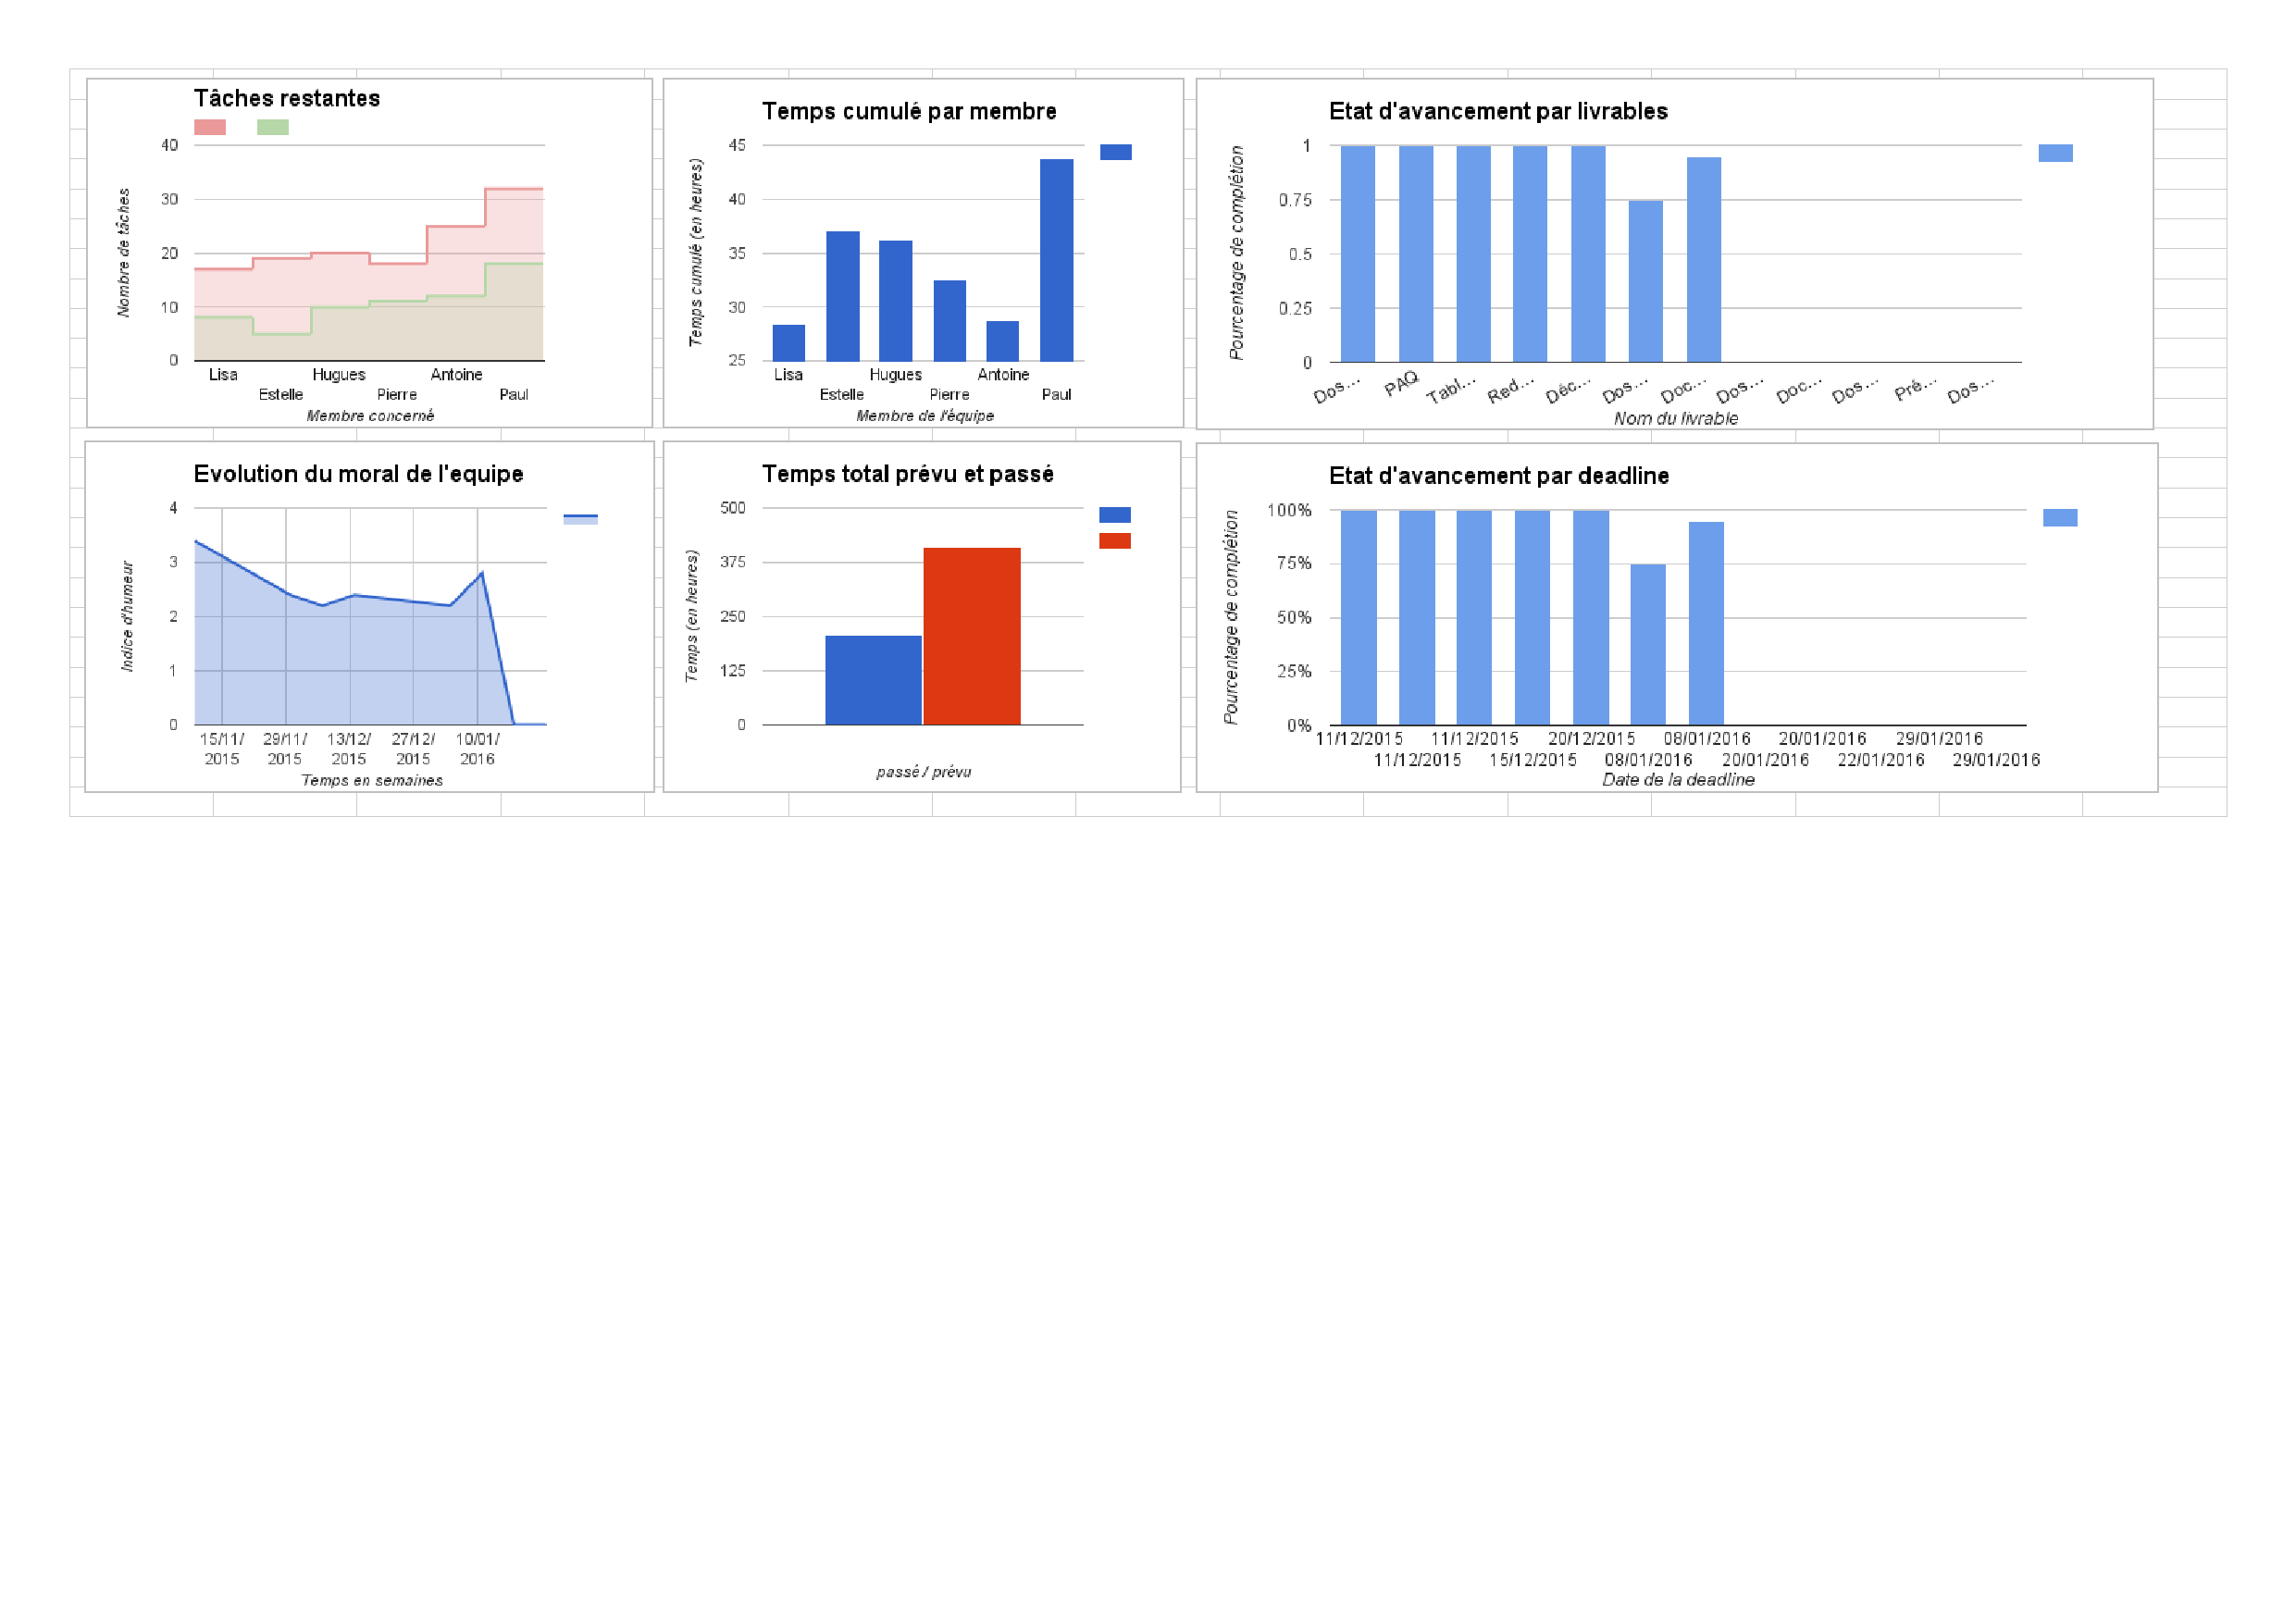
\includepdf[pages=-]{tdbs/Tableau_de_Bord_08-01-16.pdf}

\chapter{Tableau de Bord le 12/01/2016}
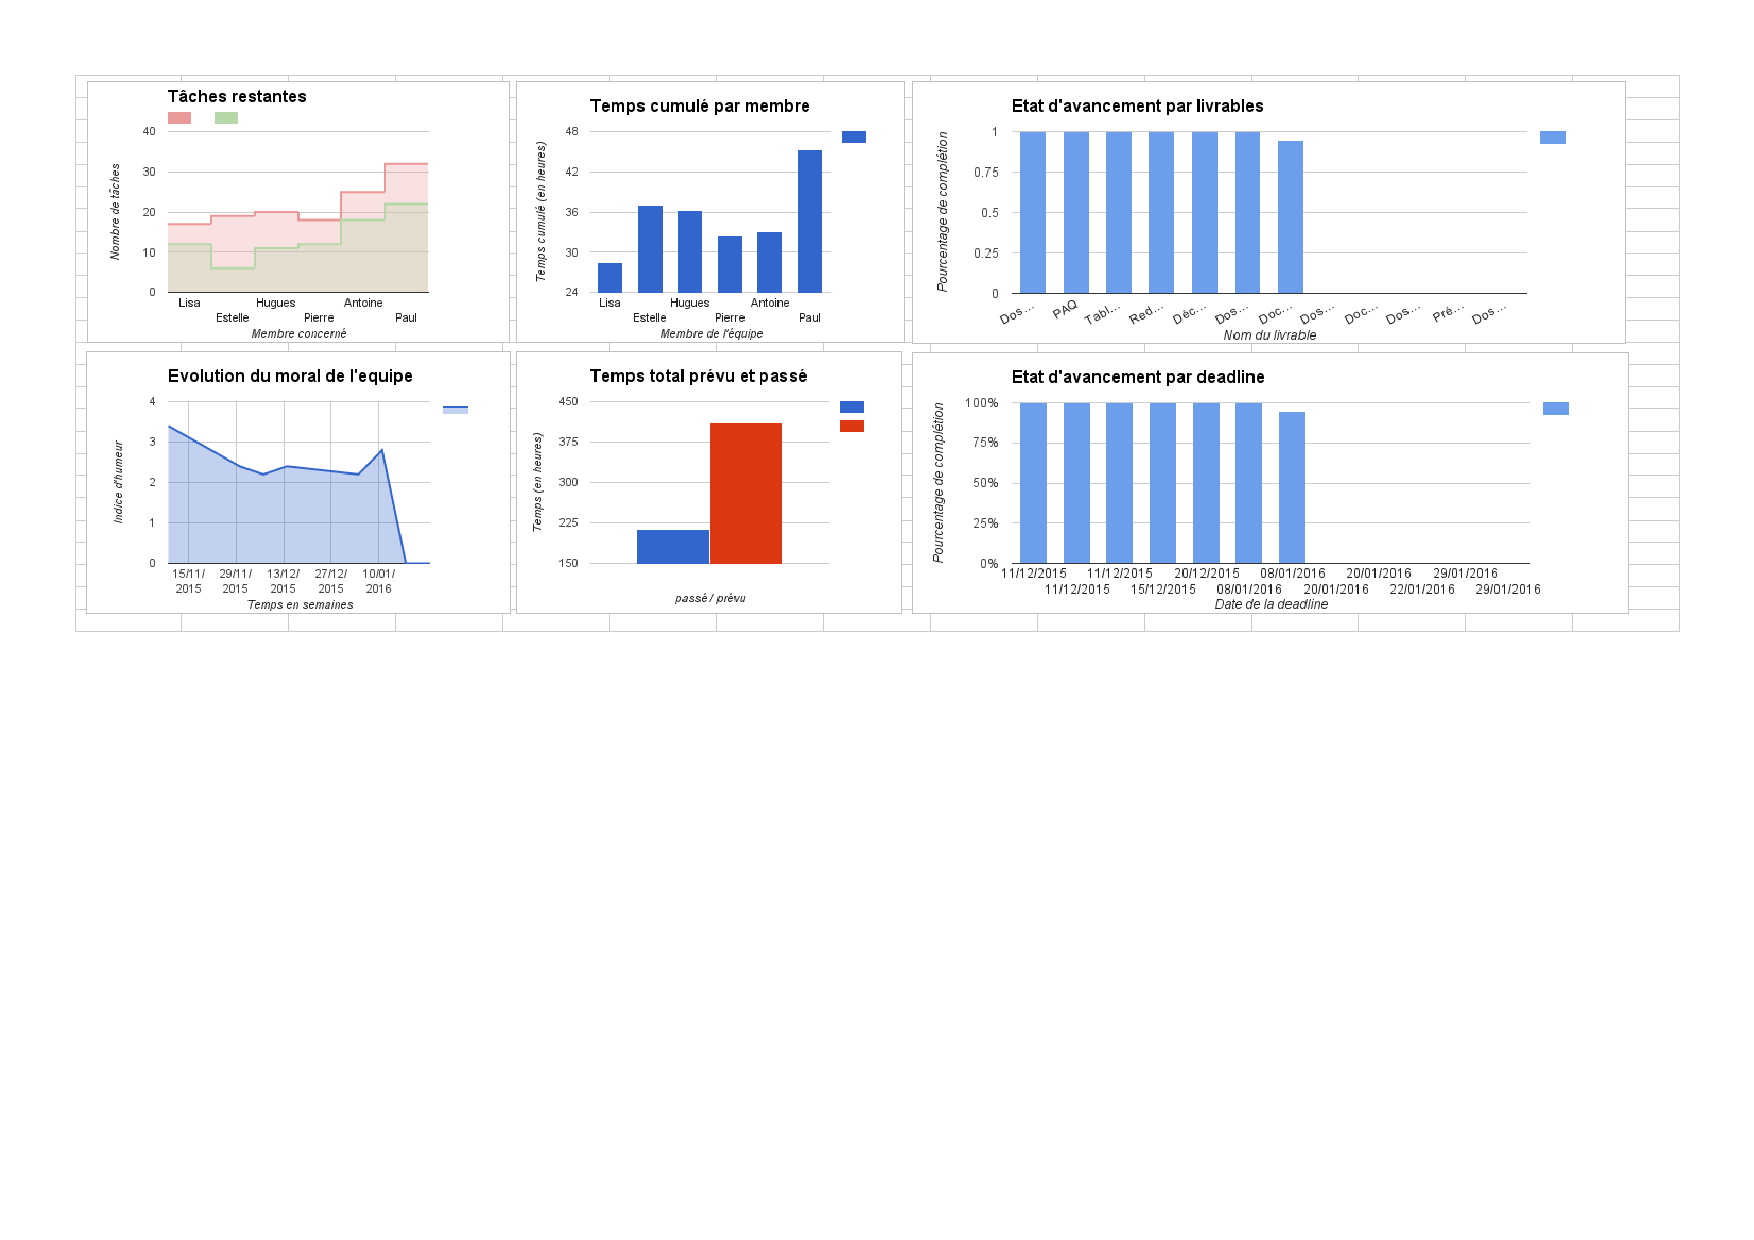
\includepdf[pages=-]{tdbs/Tableau_de_Bord_12-01-16.pdf}

\chapter{Tableau de Bord le 15/01/2016}
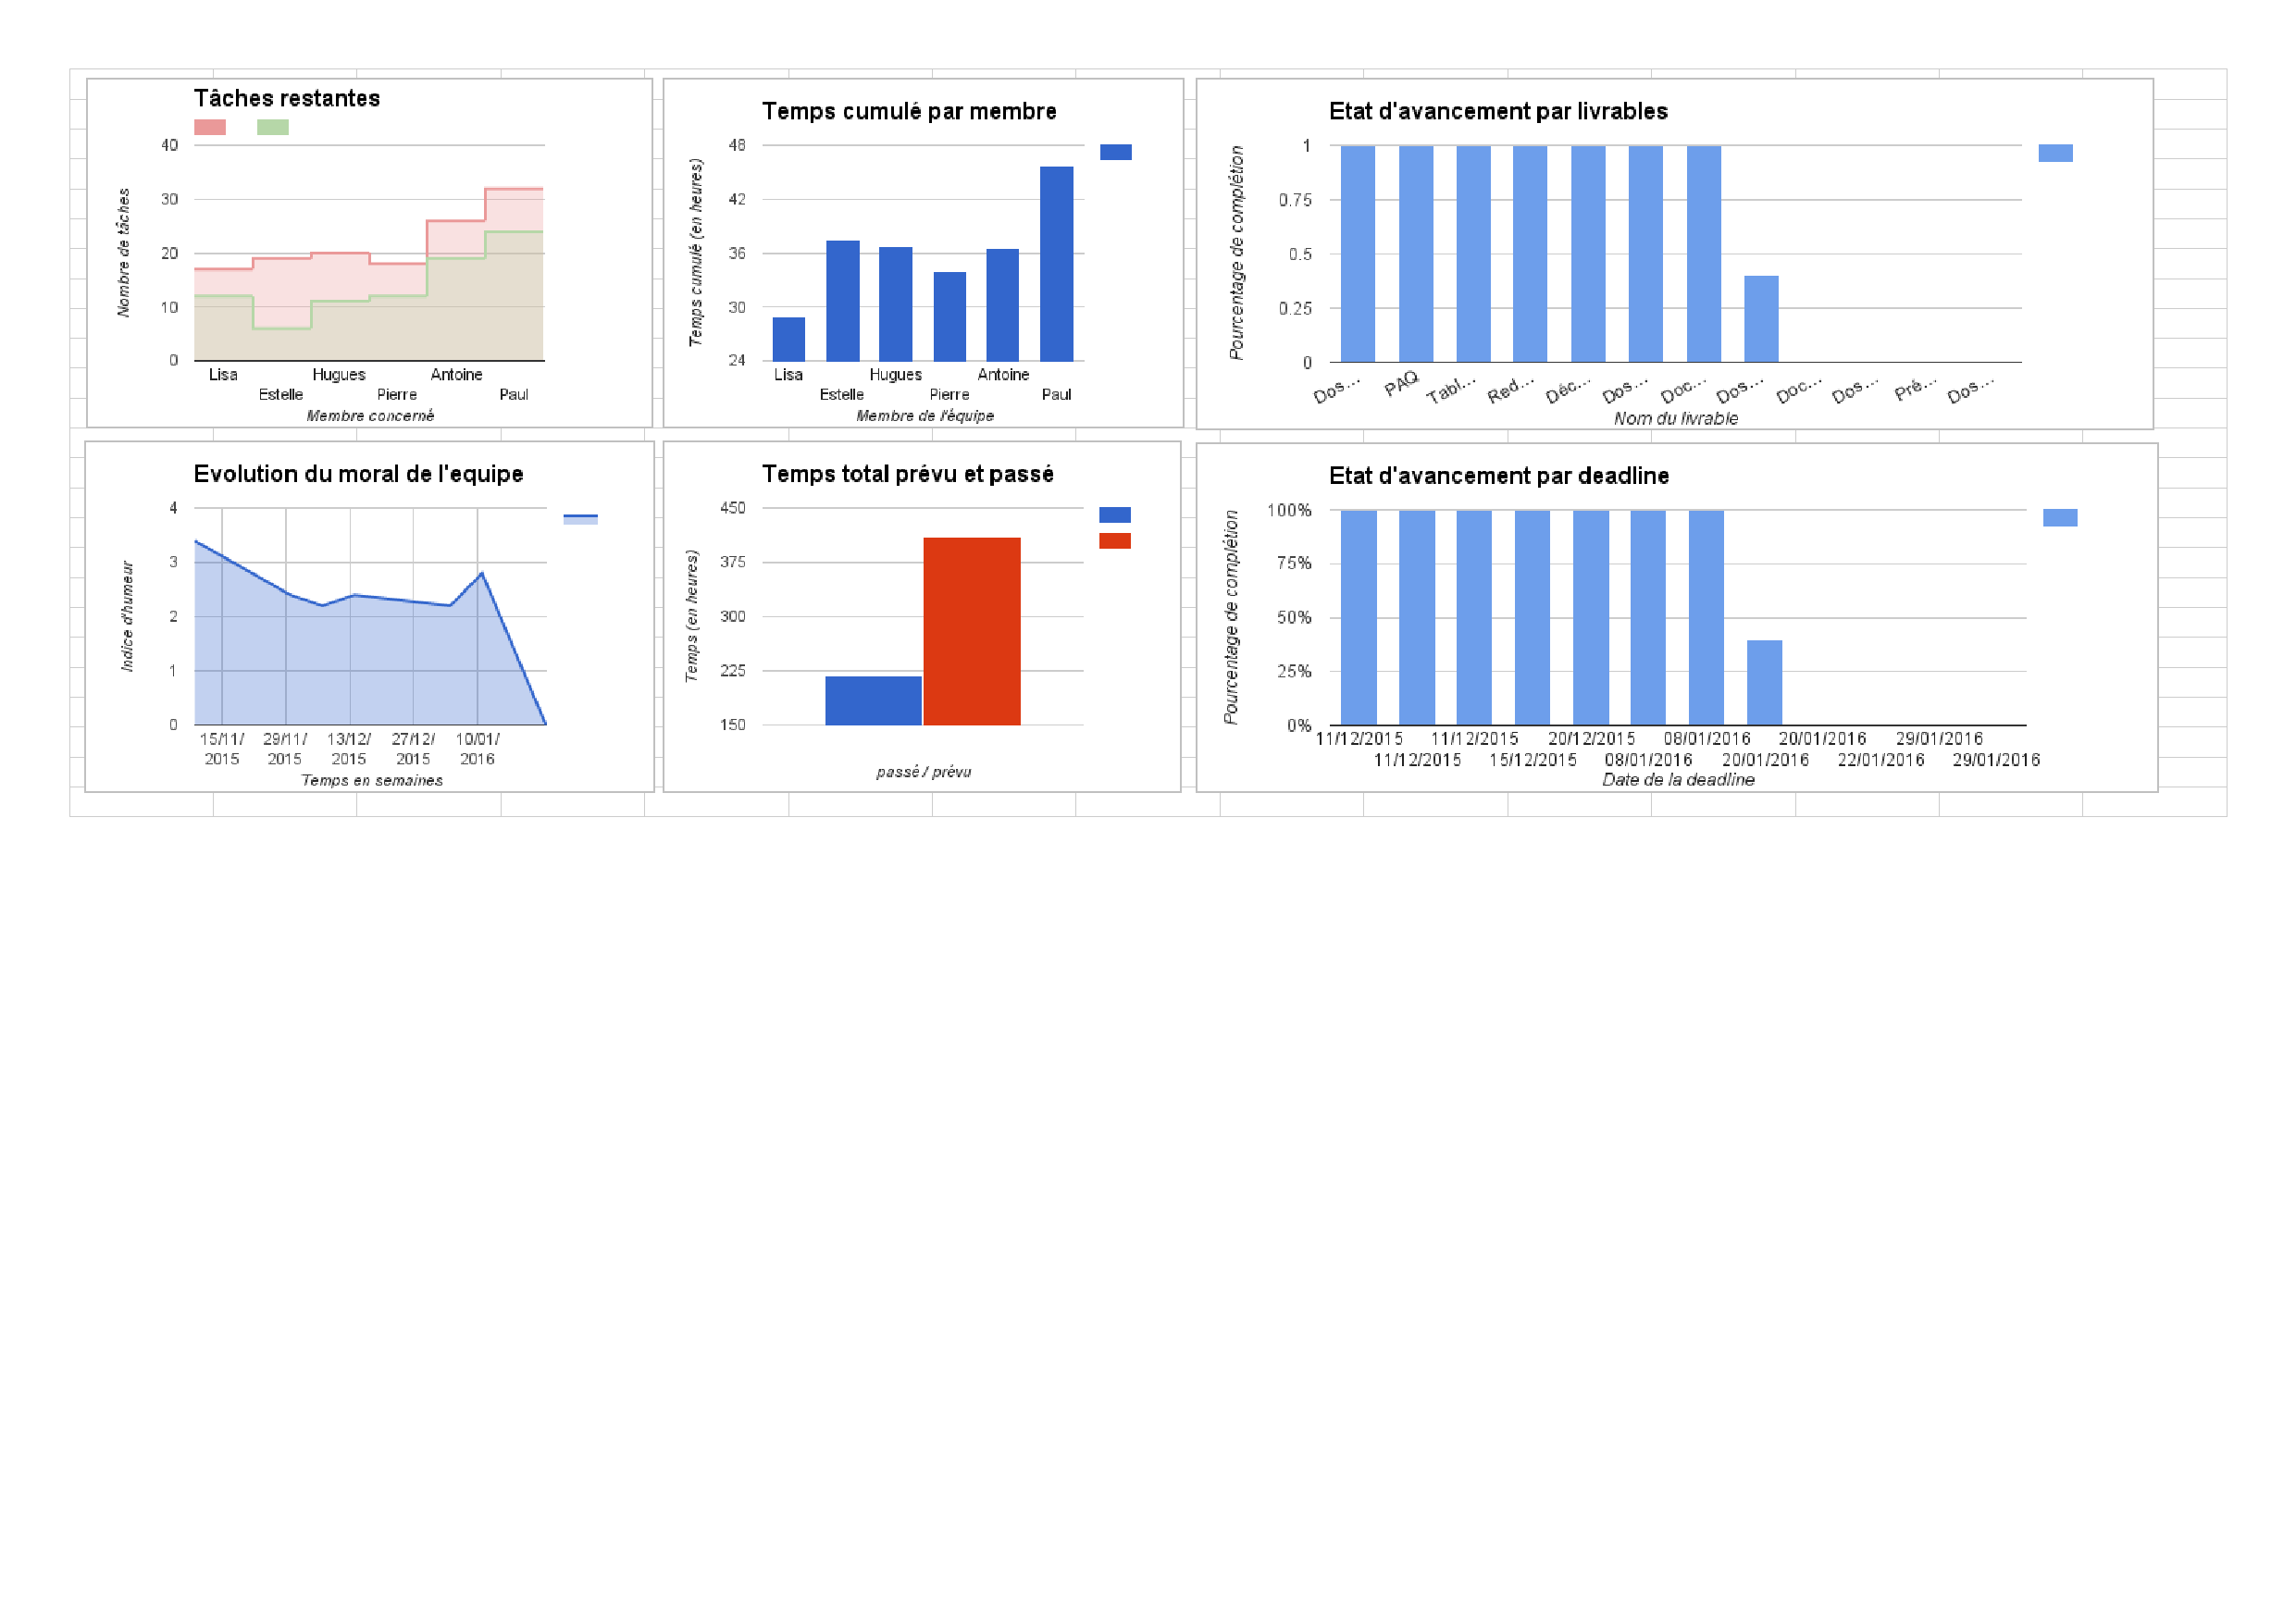
\includepdf[pages=-]{tdbs/Tableau_de_Bord_15-01-16.pdf}

\chapter{Tableau de Bord le 19/01/2016}
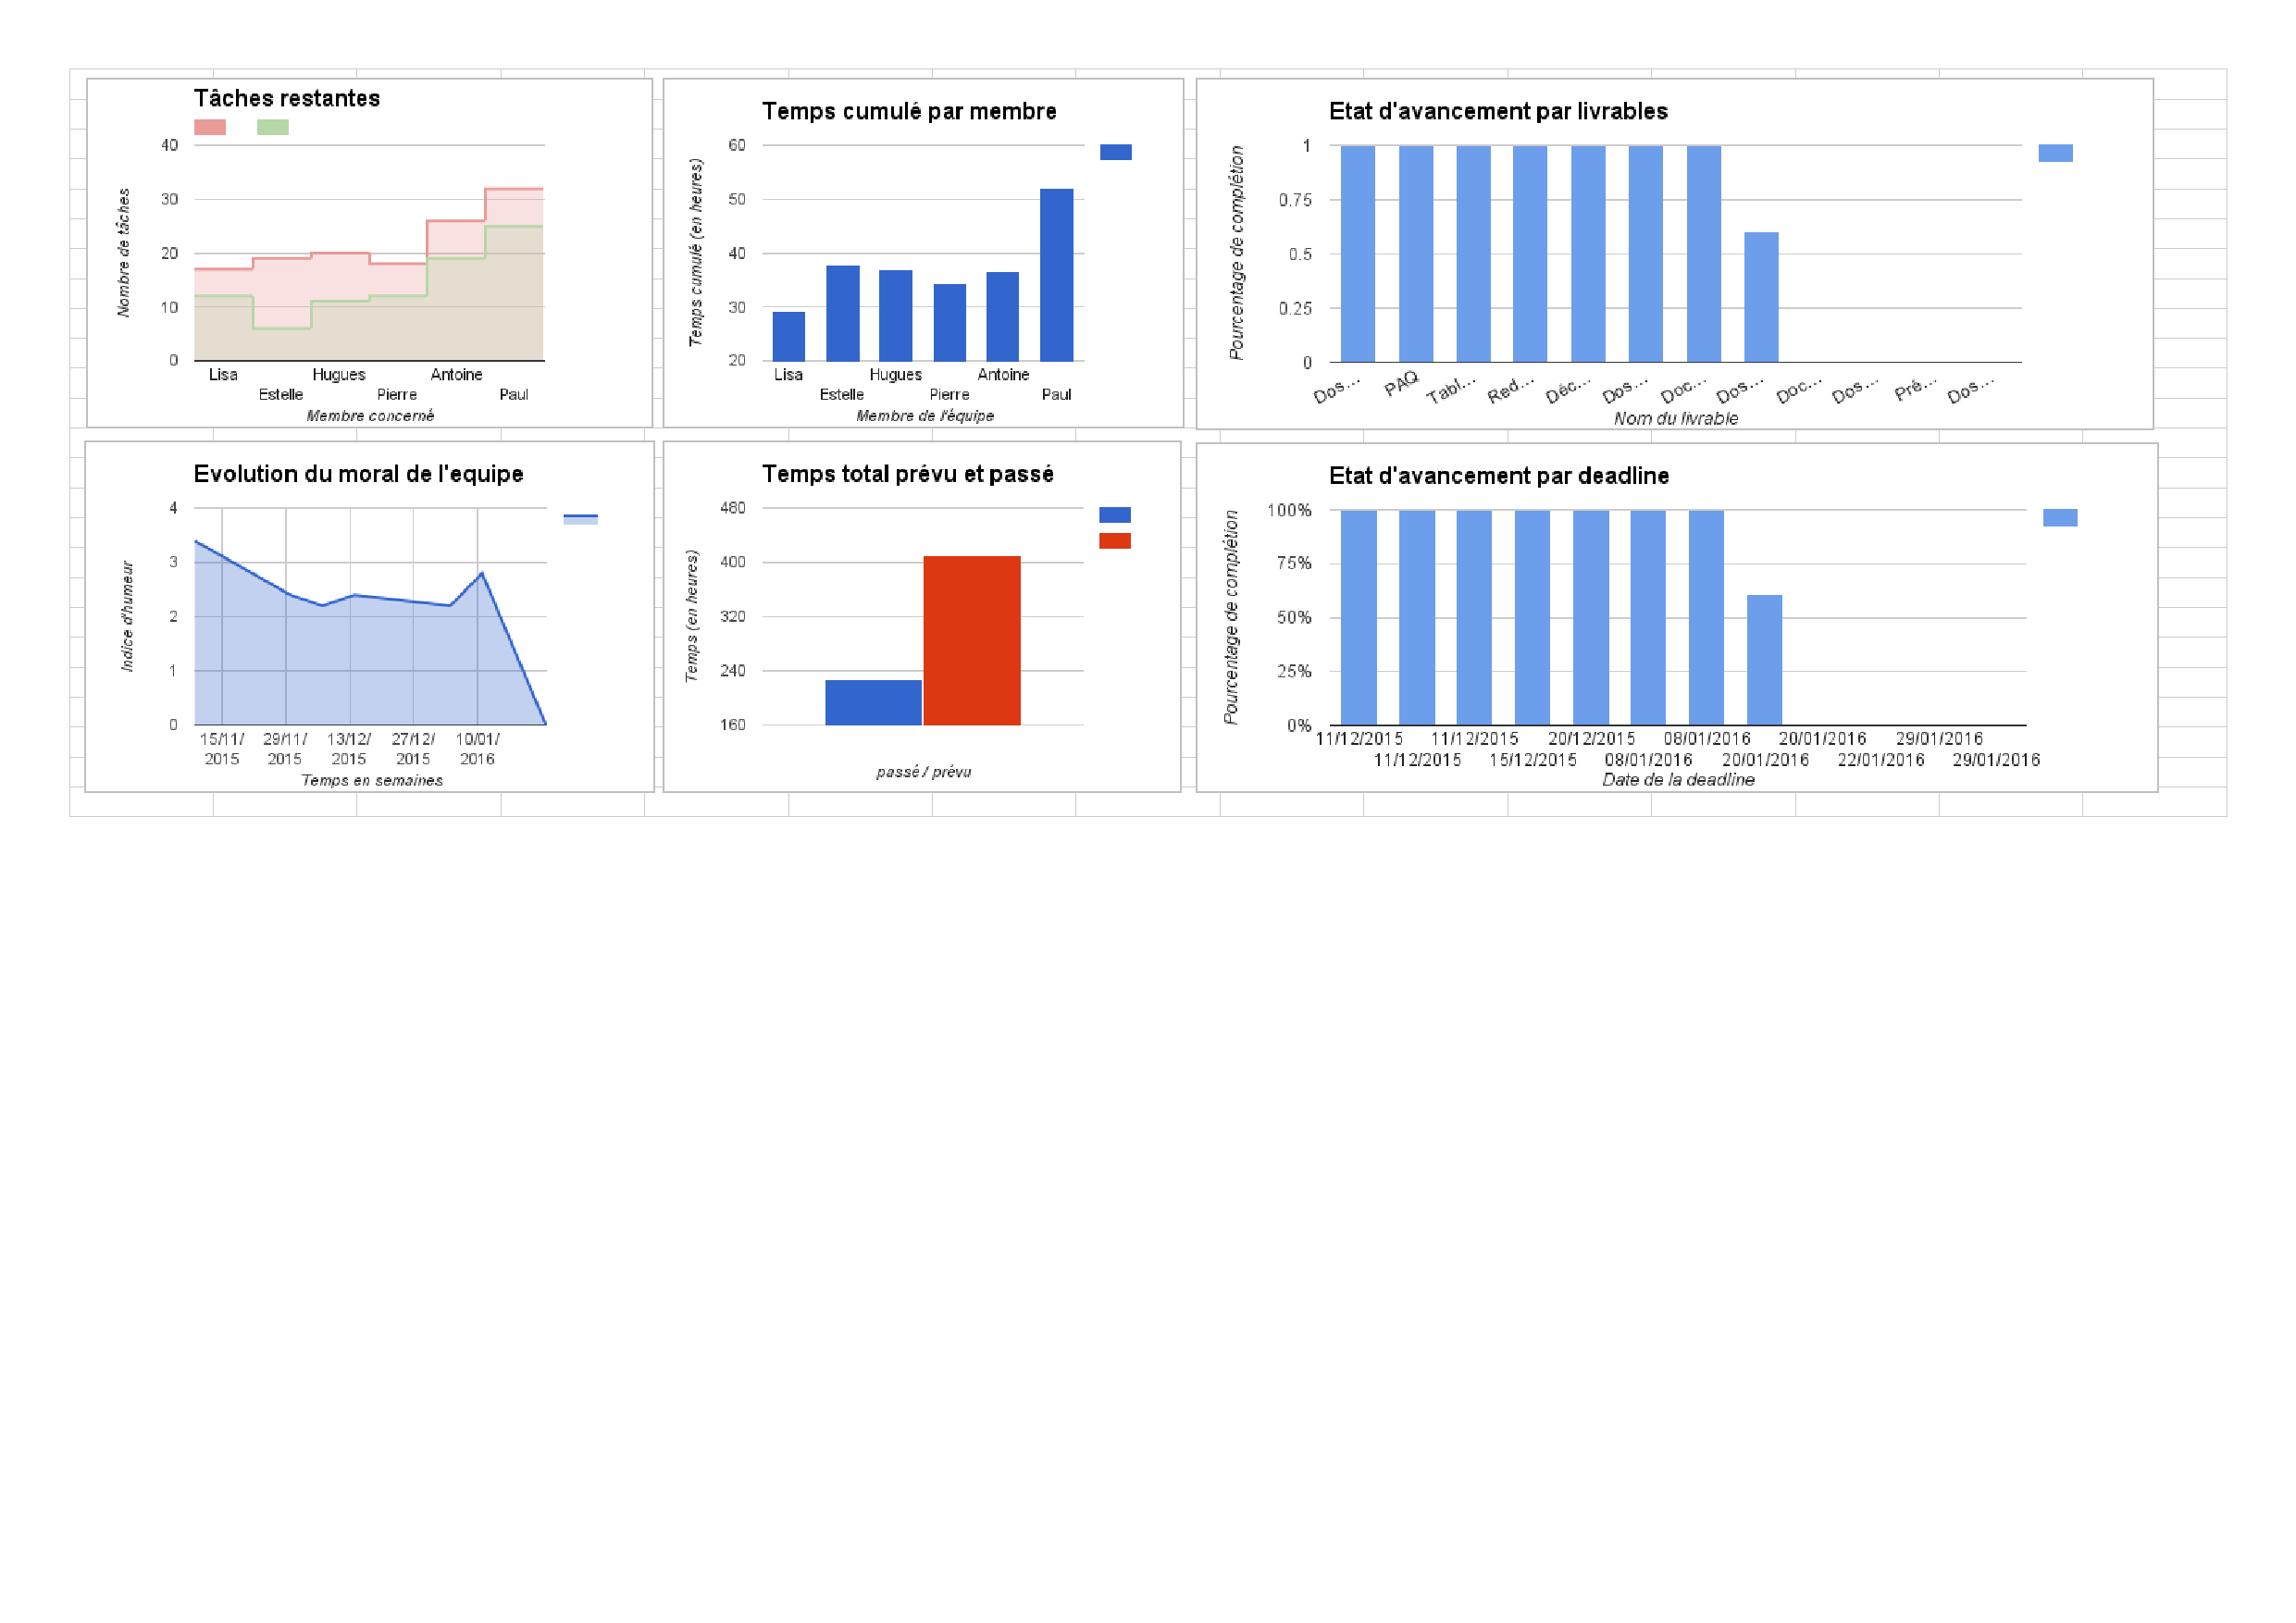
\includepdf[pages=-]{tdbs/Tableau_de_Bord_19-01-16.pdf}

\chapter{Tableau de Bord le 22/01/2016}
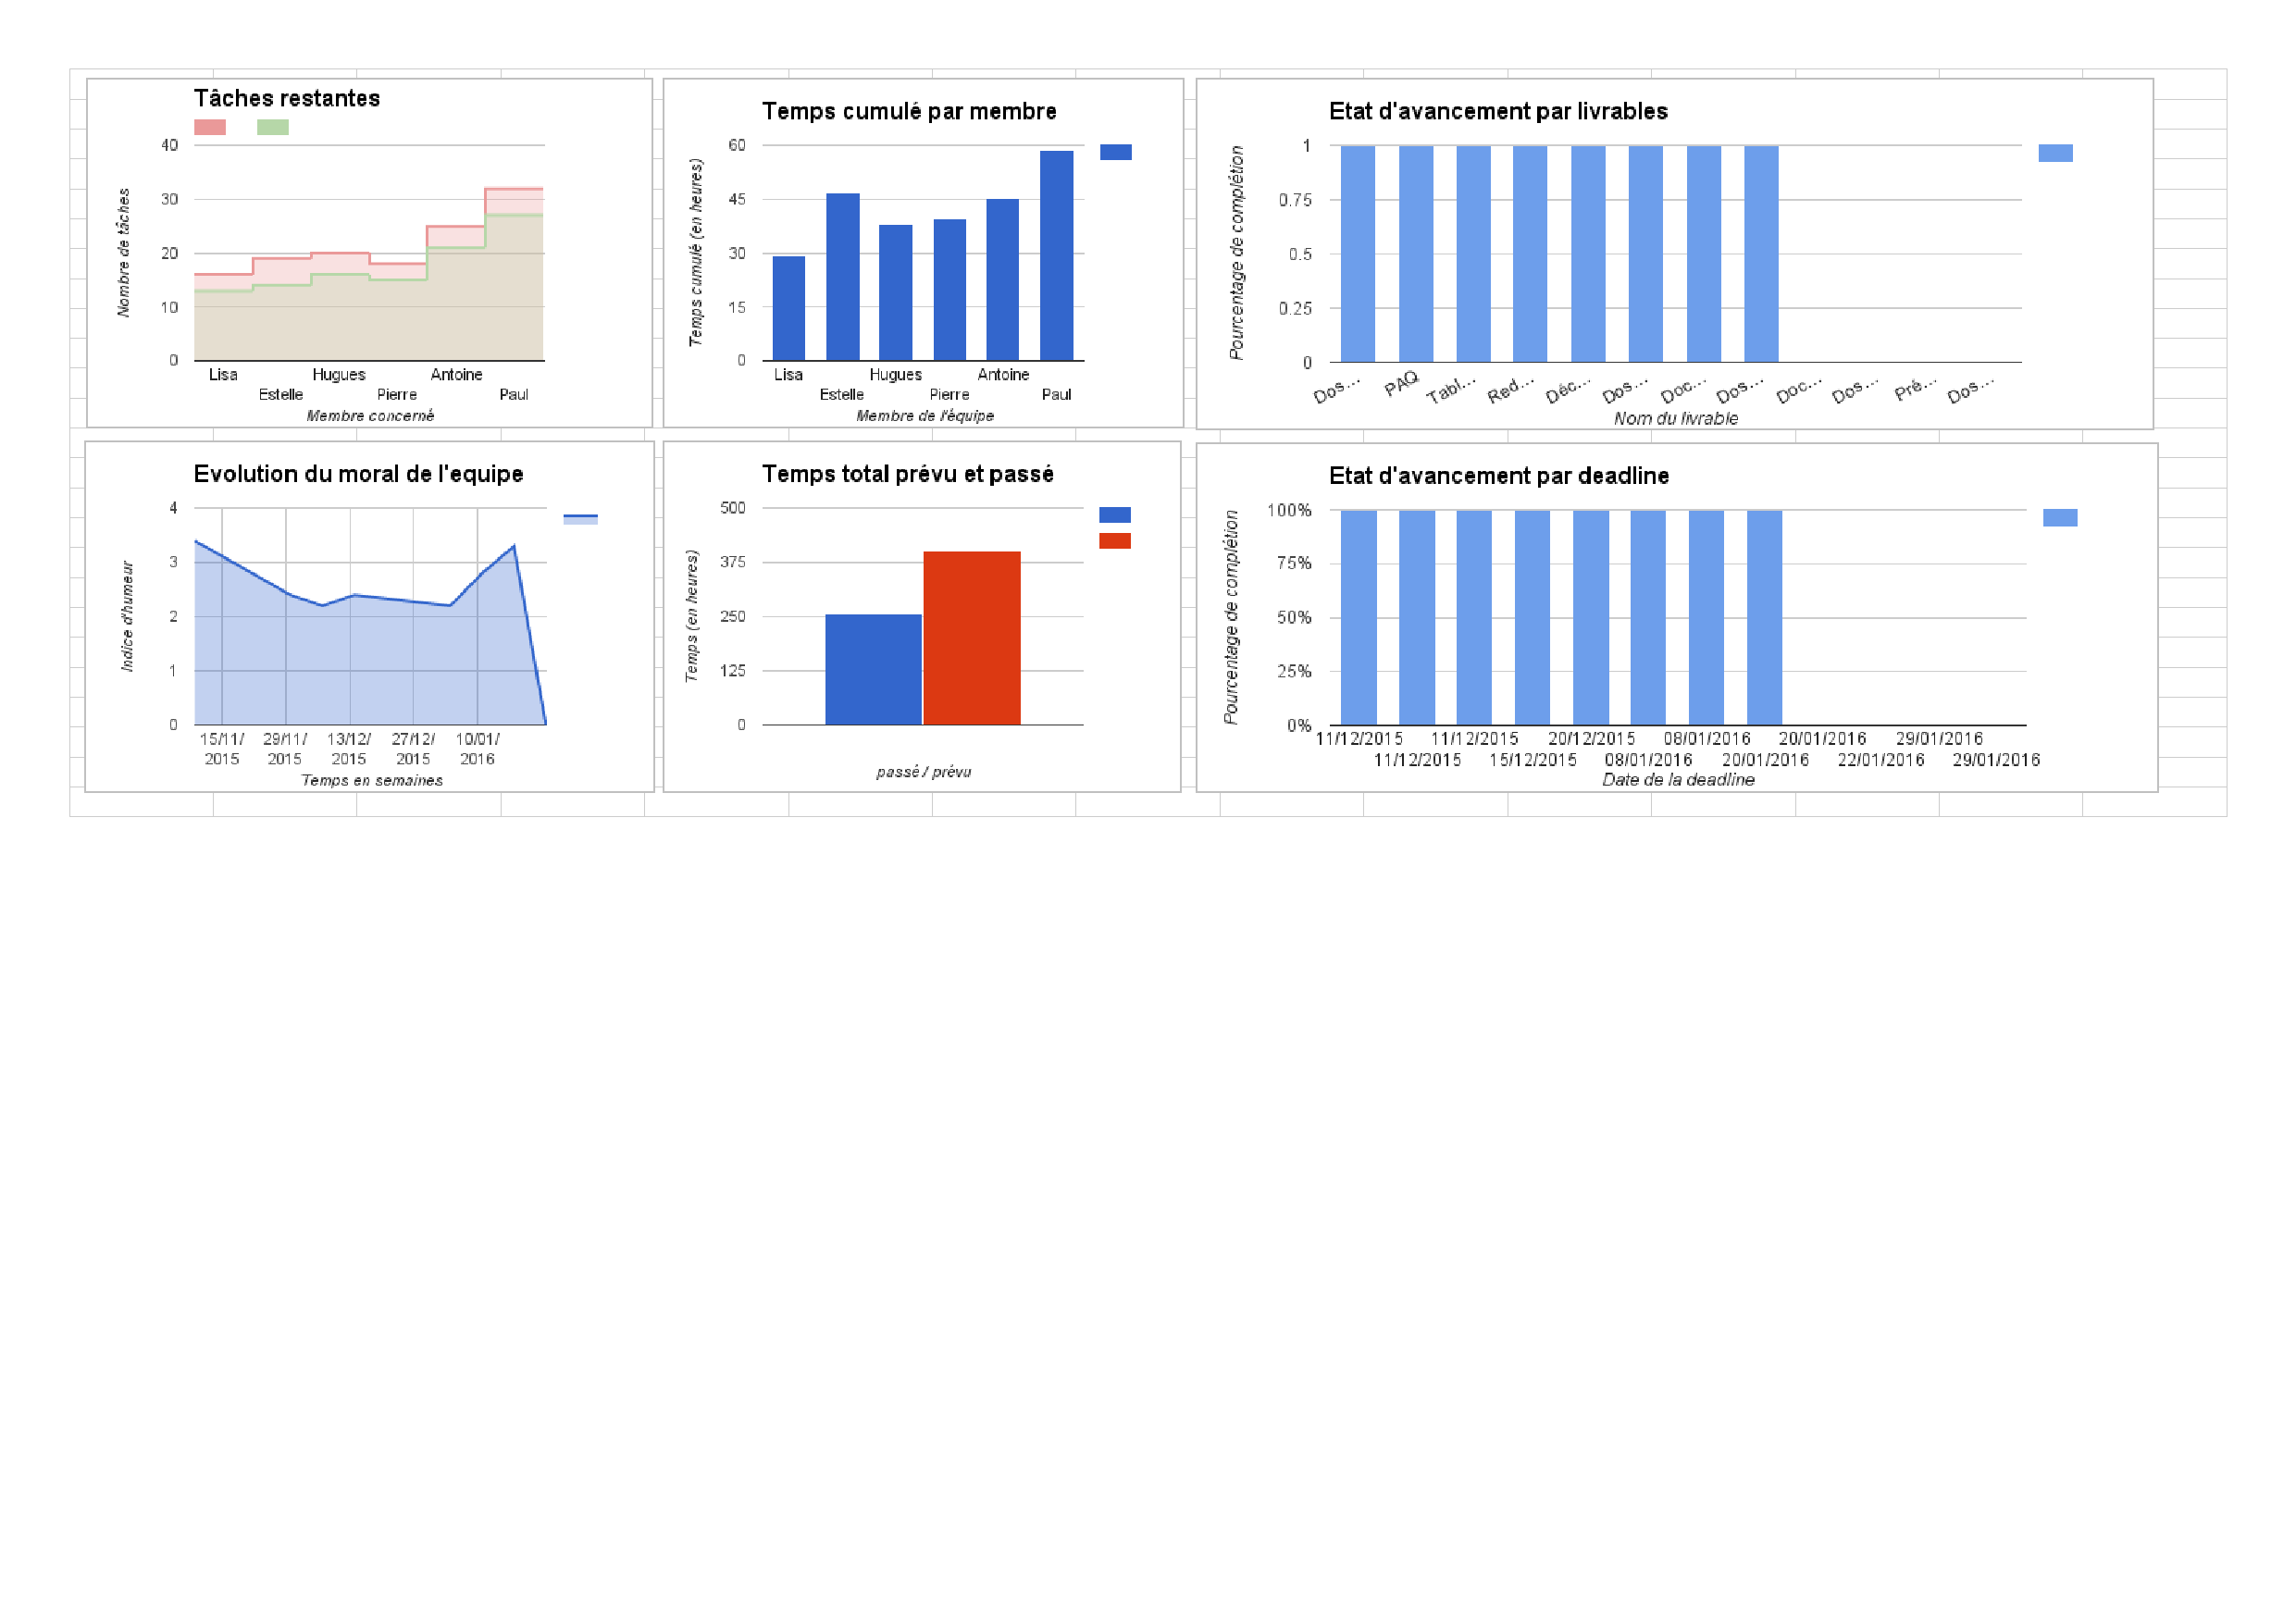
\includepdf[pages=-]{tdbs/Tableau_de_Bord_22-01-16.pdf}

\end{appendices}

%%% End document
\end{document}
